\documentclass[dvisvgm,tikz]{standalone}

\usepackage[sfdefault]{inter}
\usetikzlibrary{shapes.geometric, arrows.meta, positioning, calc, fit, decorations.pathmorphing}

%%%%%%%%%%%%%%%%%%%%%%%%%%%%%%%%%%%%%%%%%%%%%%%%%%%
%Colors
% Warm gray to turquoise
\definecolor{warm_gray}{RGB}{128, 120, 115}
\definecolor{sage_gray}{RGB}{110, 125, 120}
\definecolor{pewter}{RGB}{91, 112, 114}
\definecolor{slate_blue}{RGB}{72, 107, 115}
\definecolor{steel_teal}{RGB}{53, 118, 125}
\definecolor{teal}{RGB}{27, 136, 140}
\definecolor{deep_aqua}{RGB}{15, 152, 155}
\definecolor{peacock_blue}{RGB}{0, 167, 171}
\definecolor{blue_green}{RGB}{0, 181, 185}
\definecolor{turquoise}{RGB}{0, 195, 200}

\definecolor{mygray}{gray}{0.9}

% Match our established color scheme
\definecolor{atoken}{RGB}{255, 152, 0}        % Orange for A token
\definecolor{gtoken}{RGB}{76, 175, 80}        % Green for G token
\definecolor{mainblue}{RGB}{74, 144, 226}     % Blue for A classes
\definecolor{maingreen}{RGB}{102, 187, 106}   % Light green for G classes
\definecolor{timegray}{RGB}{158, 158, 158}    % Gray for time component
%%%%%%%%%%%%%%%%%%%%%%%%%%%%%%%%%%%%%%%%%%%%%%%%%%%

\def \G {\textbf{G}}
\def \A {\textbf{A}}
\def \Q {\textbf{Q}}
\def \C {\textbf{C}}
\def \CC {\textbf{C*}}
\def \KA {\textbf{KLIMA}}
\def \KG {\textbf{KlimaX}}

\def \AG {$\overline{\textbf{AG}}$}
\def \AQ {$\overline{\textbf{AQ}}$}

\begin{document}
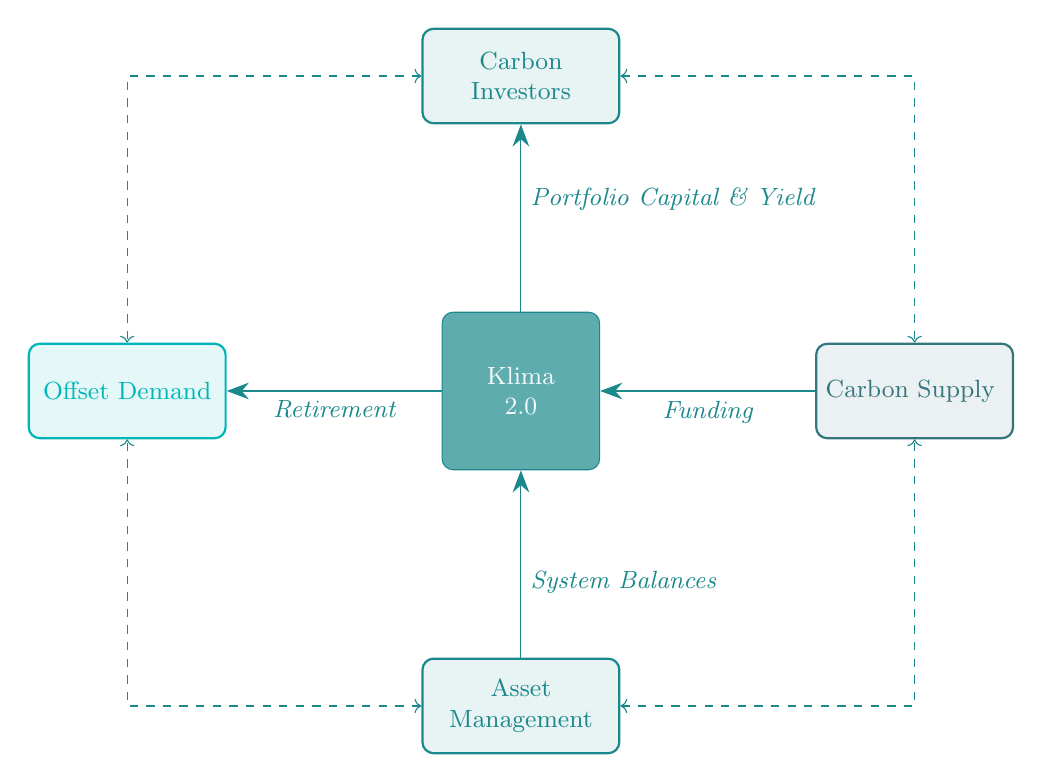
\begin{tikzpicture}[
    % Node styles
    trader/.style={
        rectangle, 
        draw=#1,
        fill=#1!10,
        text=#1,
        thick,
        rounded corners,
        minimum width=2.5cm,
        minimum height=1.2cm,
        align=center,
        font = \small
    },
    k2/.style={
        rectangle,
        draw=#1,
        fill=#1!70,
        text=#1!05,
        minimum size=2cm,rounded corners,
        align=center,
        font = \small
    },
    arrow/.style={
        -{Stealth[length=8pt]},
        thin,
        #1
    },
    dash_arrow/.style={
        -{Stealth[length=8pt]},
        thin,dashed,
        <->,
        #1
    }
]



% Position nodes
\node[trader=teal] (investor) at (0,4) {Carbon \\ Investors};

\node[k2=teal] (k2) at (0,0) {Klima \\ 2.0};

\node[trader=blue_green] (buyer) at (-5,0) {Offset Demand};

\node[trader=steel_teal] (seller) at (5,0) {Carbon Supply };

\node[trader=teal] (risk) at (0,-4) {Asset \\ Management };

% draw arrows
\draw[arrow=teal] (k2.north) -- node[pos=0.6, right, text=teal, font=\small\itshape] {Portfolio Capital \& Yield}  (investor.south);

\draw[arrow=teal] (k2.west) -- node[pos=0.5, below, text=teal, font=\small\itshape] {Retirement}  (buyer.east);


\draw[arrow=teal] (seller.west) -- node[pos=0.5, below, text=teal, font=\small\itshape] {Funding}  (k2.east);

\draw[arrow=teal] (risk.north) -- node[pos=0.4, right, text=teal, font=\small\itshape] {System Balances}  (k2.south);

\draw[dash_arrow=teal] (investor.east) -|   (seller.north);
\draw[dash_arrow=teal] (investor.west) -|   (buyer.north);

\draw[dash_arrow=teal] (risk.east) -|   (seller.south);
\draw[dash_arrow=teal] (risk.west) -|   (buyer.south);

\end{tikzpicture}
\end{document}
